\usetheme{Warsaw}
\definecolor{mucyellow}{RGB}{255,235,0}
\definecolor{mucblack}{RGB}{0,0,0}

\setbeamercolor{structure}{fg=mucblack}

\setbeamercolor{palette primary}{fg=mucblack,bg=mucyellow!70}
\setbeamercolor{palette secondary}{fg=mucblack,bg=mucyellow!80}
\setbeamercolor{palette tertiary}{fg=mucblack,bg=mucyellow!90}
\setbeamercolor{palette quaternary}{fg=mucblack,bg=mucyellow}

\setbeamercolor{titlelike}{parent=palette quaternary}

\setbeamercolor{block title}{fg=mucblack,bg=mucyellow}
\setbeamercolor{block title alerted}{use=alerted text,fg=mucblack,bg=alerted text.fg!75!bg}
\setbeamercolor{block title example}{use=example text,fg=mucblack,bg=example text.fg!75!bg}

\setbeamercolor{block body}{parent=normal text,use=block title,bg=block title.bg!25!bg}
\setbeamercolor{block body alerted}{parent=normal text,use=block title alerted,bg=block title alerted.bg!25!bg}
\setbeamercolor{block body example}{parent=normal text,use=block title example,bg=block title example.bg!25!bg}

\setbeamercolor{sidebar}{bg=mucyellow!70}
\setbeamercolor{palette sidebar primary}{fg=mucblack}
\setbeamercolor{palette sidebar secondary}{fg=mucblack!75}
\setbeamercolor{palette sidebar tertiary}{fg=mucblack!75}
\setbeamercolor{palette sidebar quaternary}{fg=mucblack}

\setbeamercolor*{separation line}{}
\setbeamercolor*{fine separation line}{}

\setbeamertemplate{headline}[default]
\AtBeginSection[]
{
 \begin{frame}
  \frametitle{Fahrplan}
  \tableofcontents[currentsection,hideothersubsections]
 \end{frame}
}

\addtobeamertemplate{navigation symbols}{}{%
    \usebeamerfont{footline}%
    \usebeamercolor[fg]{footline}%
    \hspace{1em}%
    \insertframenumber/\inserttotalframenumber
}

\setbeamertemplate{background}{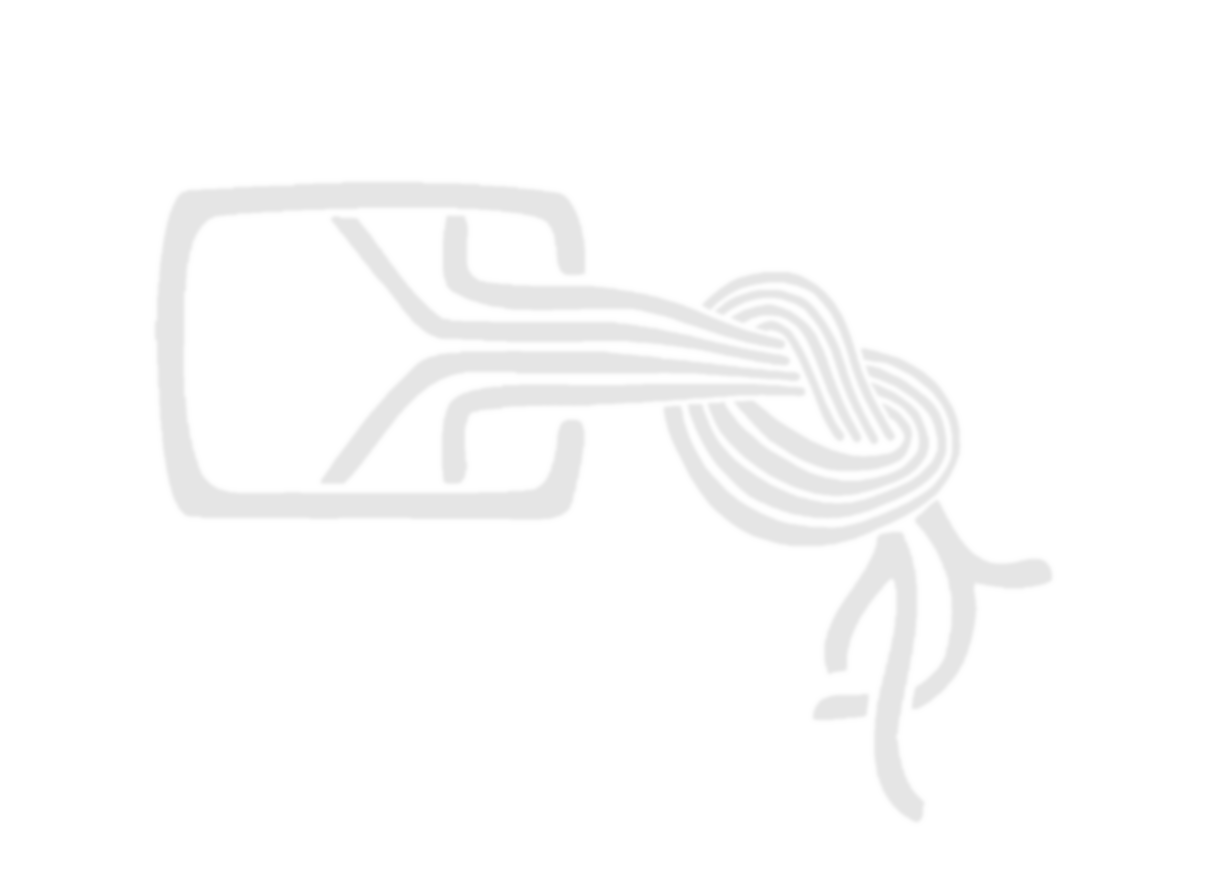
\includegraphics[width=\paperwidth,height=\paperheight]{images/chaosbrezn.png}}

